\documentclass[10pt]{article}
\usepackage[polish]{babel}
\usepackage[utf8]{inputenc}
\usepackage[T1]{fontenc}
\usepackage{amsmath}
\usepackage{amsfonts}
\usepackage{amssymb}
\usepackage[version=4]{mhchem}
\usepackage{stmaryrd}
\usepackage{graphicx}
\usepackage[export]{adjustbox}
\graphicspath{ {./images/} }

\title{Zadania - etap III (FINAŁ) }

\author{}
\date{}


\begin{document}
\maketitle
CENTRUM NAUCZANIA MATEMATYKI\\
I KSZTAŁCENIA NA ODLEGŁOSĆ

Zadanie 1. (5p.) Na bokach \(A B\) i \(B C\) trójkąta równobocznego \(A B C\) zbudowano - odpowiednio - kwadrat i trójkąt równoboczny tak, jak na poniższym rysunku. lle wynosi miara kata CNK ?\\
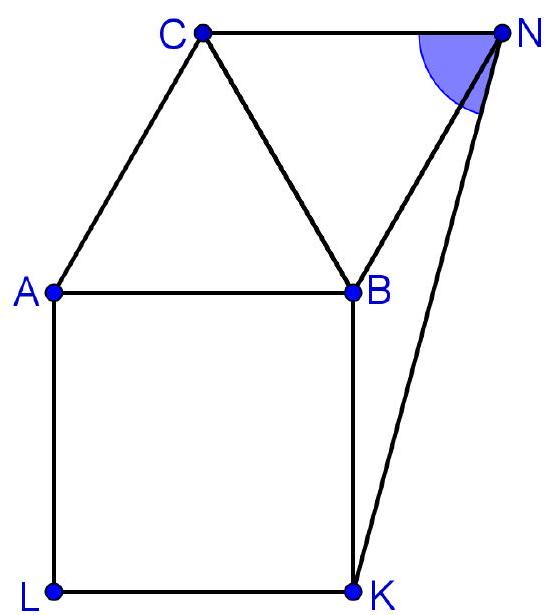
\includegraphics[max width=\textwidth, center]{2024_11_21_802b58213c5ab9fa2b63g-1}

Zadanie 2. (5p.) Pan Kowalski ma kilkoro dzieci. Wiemy, że iloczyn liczb wyrażajacych wiek dzieci (w latach) wynosi 1664 oraz, że najstarsze dziecko jest dwa razy starsze od najmłodszego. Ile dzieci ma pan Kowalski?

Zadanie 3. (5p.) Tadek wybrał trzy liczby: \(a, b, c\) i zauważył, że ich iloczyn wynosi 360. lloczyn dwóch pierwszych liczb wynosi 90, zaś iloczyn drugiej i trzeciej liczby wynosi 120. Jakie liczby wybrał Tadek?

Zadanie 4. (5p.) W prostokacie \(A B C D\) długość boku \(B C\) stanowi \(\frac{3}{8}\) długości boku \(A B\). Z wierzchołka \(A\) poprowadzono odcinek do środka boku \(C D\). Odcinek ten podzielił prostokąt \(A B C D\) na dwie figury: trapez o obwodzie 20 cm i trójkąt o obwodzie 12cm. Ile wynoszą długości boków prostokąta \(A B C D\) ?

Zadanie 5. (5p.) W pewnej klasie na planecie Dragon X/C sa smoki i smoczyce. Wiadomo, że smoki i smoczyce maja po 4 łapy. Każdy smok ma 4 głowy, a każda smoczyca ma 3 głowy. W szatni przed lekcja smoki i smoczyce zostawiły czapki i kalosze. lle jest smoków i smoczyc w tej klasie, jeśli w szatni znajduje się 38 czapek i 44 sztuki kaloszy?


\end{document}